% Author: Elena Marochkina <xmaroc00@stud.fit.vutbr.cz>
% Author: Nikita Pasynkov <xpasyn00@stud.fit.vutbr.cz>

\documentclass[11pt, a4paper]{article}

\usepackage[czech]{babel}
\usepackage[utf8]{inputenc}
\usepackage[T1]{fontenc}
\usepackage[left=2cm, top=3cm, text={17cm, 24cm}]{geometry}
\usepackage{times}
\usepackage{graphicx}
\usepackage{pdflscape}

\begin{document}
\begin{titlepage}
\begin{center}
    \includegraphics[width=0.77 \linewidth]{FIT_logo.pdf} \\
    \vspace{\stretch{0.382}}
    \Huge{Projekt 1.~část} \\
    \Huge{Datový model (ERD) a model případů užití} \\
    \Large{\textbf{Zadání č.~40.\,--\, Internetový obchod}} \\
    \Large{Databázové systémy}
    \vspace{\stretch{0.618}}
\end{center}

{\Large
    \today
    \hfill
    \begin{tabular}{l l}
		Nikita Pasynkov & (xpasyn00) \\
		Elena Marochkina & (xmaroc00) \\
    \end{tabular}
}
\end{titlepage}

% Obsah %
\pagenumbering{roman}
\setcounter{page}{1}
\tableofcontents
\clearpage

% Zadání %
\pagenumbering{arabic}
\setcounter{page}{1}

\section{Zadání}
Cílem je vytvoření jednoduché aplikace pro internetový obchod s určitým druhem zboží např. knihkupectví. Návštěvníci WWW stránek mají možnost prohlížet si veškerý sortiment obchodu, který je členěn do kategorií, ať už daný produkt je skladem či nikoliv. Pokud má návštěvník zájem o určitý produkt, může si jej vybrat (vložení do nákupního košíku). Vybrané zboží si může objednat po zadání potřebných údajů (kontakt, doprava, ...). Zboží si může objednat pouze registrovaný uživatel, pokud uživatel nakupuje poprvé, musí se zaregistrovat a získá přihlašovací jméno a heslo. Tyto údaje může použit k modifikaci osobních informací. Po zaplacení zákazníkem za zboží je považována obchodní transakce za vyřízenou a zaměstnanec obchodu vyexpeduje zboží podle objednávky. Vedení obchodu má informace o celkových tržbách, oblíbenosti zboží, jeho kapacitě, o objednávkách, kdo ji vyřizoval atd.
% Datový model (ERD) %
\newpage
\begin{landscape}
\section{Datový model (ERD)}
 \begin{figure}[!ht]
    \centering
    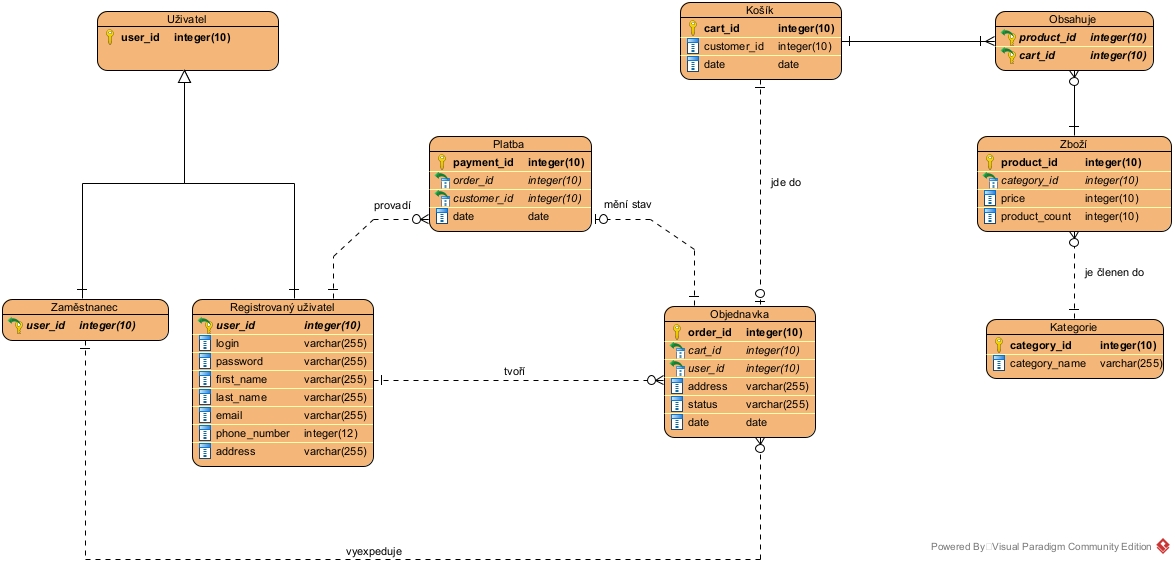
\includegraphics[width=1\linewidth]{IDS - project_1.jpg}
    \caption{Datový model (ERD)}
    \label{figure:ast_example1}
\end{figure}

\end{landscape}

% Datový model (ERD) %
\newpage
\section{Model případů užití}
 \begin{figure}[!ht]
    \centering
    \includegraphics[width=1\linewidth]{}
    \caption{Model případů užití}
    \label{figure:ast_example1}
\end{figure}
\end{document}
